% !TEX root = ../main.tex
%
\chapter{Experiments and Results}
\label{sec:evaluation}


\section{Experimental Setup}
\label{sec:evaluation:experimental}

\subsection{Synthetic Dialogue Creation}
\label{ssec:evaluation:experimental-dialogue}

We initially run the SDF with the following configurations:

\begin{enumerate}
	\item Select a controversial topic from Table \ref{tab:topics}.
	
	\item Select names and SDBs for user 1 and user 2. A full list of SDBs used can be found in Table \ref{tab:user-sdbs}
	
	\item Select whether a moderator is present.
	
	\item Provide actors with the global context.
	
	\item Provide user and moderator instructions according to the prompting strategy used (see Section \ref{sec:system:design-prompt}).
	
	\item Pick conversation configurations such as context length, conversation length e.t.c.
\end{enumerate}

The combination of the settings above produces a set of JSON configuration files, each containing the configuration for a single experiment. We execute all possible combinations, with the exception of "freezing" conversation-specific configurations. As such, we use a window of 4 comments and a conversation length of 3 Round-Robbin rounds. It is worth noting that we also avoid pitting the African American SDB against the LGBTQ+ SDB.

\begin{table}
	\begin{tabular}{@{\makebox[3em][r]{\rownumber\space}} | p{0.8\linewidth}}
		Homosexuality, transgender sex all are deviations from normal human behavior as well. \\
		\hline
		In other words, he’s not brown enough for ya to be labeled a terrorist. \\
		\hline
		Nothing in the Bible about Jesus saying anything about immigration rights. [...] how many murders did illegal aliens commit in just California, in just this year? Just California. How many murders by illegal aliens? You answer that.\\
		\hline
		Are you high??? Selling someone a cake? Refusing to sell some a cake because it is for a gay wedding is no different from selling someone a cake because it is for a mixed race wedding or a Muslim wedding or any other kind of wedding. IT IS DISCRIMINATION! Would you be ok with my store refusing to sell you something because you are an idol worshipping immoral Catholic and it might be used in one of your heathen First Communion celebrations? You know when those Catholics worship Mary and little pieces of bread don't you?\\
		\hline
		How do you know he is not proud of his cakes? Artists do not take pride in their work? Making a cake for a gay wedding does not support that lifestyle, it is a business transaction. Period. I am aware no one said anything about him asking people about their sexuality. I am sorry that was hard for you to understand. Is he going to ask everyone that comes in if the cake is for a gay wedding? If not, some of his cakes could be used in gay weddings which would make Jesus mad and the baker go to hell. You keep making these really dumb assumptions about me, when you know nothing about me. I am not confused, you are rude. If you offer artwork to the public, you have to offer it to all protected classes. Why would black people be discriminated against? Precedent. Ridiculous? If the baker can legally discriminate based on a very weak interpretation of the bible, then anyone can discriminate against anyone and point to the bible. Satanists can discriminate against Christians...\\
		\hline
		well thats a no brainer hillary clinton gave huma abdein a security clearance when she has ties to a known terrorist group the muslim brotherhood, and her mother runs an anti american news paper in the middle east, debbie washed up crook shultz got the awan famaily security clearances and they were recent immigrants, had absolutely no IT experience and possible ties to terrorist groups in pakistan. its pretty clear our liberal ran government is a complete and total failure when it comes to national security. 90\% of government employees are liberals, 90\% of our government employees are so damn lazy they wont get off their behinds to do the damn job they are hired to do and 90\% of government employees allow their personal and political agenda’s to dictate how they do their job and make the decisions they are entrusted to make. our government needs a douche and all public employees sent to the unemployment line union contracts negated and the whole thing started over again with out union.\\
		\hline
		All men are sex offenders? Really? A sexual predator is a person who attacks a victim. Typical men don’t rape or use force on women. You are obviously a person who hates men and or healthy, normal sex.\\
		\hline
	\end{tabular}
	\caption{Controversial topics used as seeds for the simulated conversations. Abstracts selected from \cite{pavlopoulos-likas-2024-polarized}.}
	\label{tab:topics}
\end{table}


\begin{table}
	\begin{tabular}{@{\makebox[3em][r]{\rownumber\space}} | p{0.8\linewidth}}
		W.E.I.R.D. (Western, Educated, Industrialized, Rich, and Democratic)\\
		\hline
		A member of the LGBTQ+ community \\
		\hline
		An African American\\
		\hline
	\end{tabular}
	\caption{SDBs given to LLM users during the production of synthetic dialogues.}
	\label{tab:user-sdbs}
\end{table}


\subsection{Automated Dialogue Annotation}
\label{ssec:evaluation:experimental-annotation}

For each produced synthetic dialogue we pick one out of the annotator SDBs present in Table \ref{tab:annotator-sdbs}. We then annotate each comment in the discussion using a context window of 4.


\begin{table}
	\begin{tabular}{@{\makebox[3em][r]{\rownumber\space}} | p{0.8\linewidth}}
		No SDB (control) \\
		\hline
		W.E.I.R.D. (Western, Educated, Industrialized, Rich, and Democratic) \\
		\hline
		A member of the LGBTQ+ community \\
		\hline
		An African American \\
		\hline
		A gamer \\
		\hline
		An elderly person \\
		\hline
		A university professor\\
		\hline
		A blue-collar worker\\
		\hline
	\end{tabular}
	\caption{SDBs given to LLM annotators during the annotation of synthetic discussions.}
	\label{tab:annotator-sdbs}
\end{table}


\section{Produced Datasets}
\label{sec:evaluation:datasets}

We produce three synthetic datasets:

\begin{itemize}
	\item The \textbf{Synthetic Dialogues Dataset}, containing the logs of the conversations, as well as rich metadata such as the prompts used and the conversation-specific configurations.
	
	\item The \textbf{Automated Annotation Dataset}, containing the annotations for each comment in each synthetic conversation. Contains metadata similar to the Synthetic Dialogues Dataset such as annotator prompt and context length.
	
	\item The \textbf{Controversial Comments Dataset}, containing the comments in which the annotators disagreed upon. Includes comment and conversation IDs for matching with the other datasets, the nDFU \cite{pavlopoulos-likas-2024-polarized} score of each comments, and the individual annotations for each annotator SDB.
\end{itemize}

Descriptive statistics for the above datasets can be found in Table \ref{tab:datasets}. Some datasets are provided in the form of sets of JSON files, in which case we use the row and column numbers from their converted form as \code{pandas dataframes}. All datasets contain primary and foreing keys in the form of unique IDs enabling the user to freely combine information from all three datasets.


\begin{table}
	\begin{tabular}
		{ |p{6cm}|p{1cm}|p{1.5cm}|p{2cm}|}
		\hline
		\cellcolor{blue!25}\textbf{Name} & \cellcolor{blue!25}\textbf{Rows} & \cellcolor{blue!25}\textbf{Columns} & \cellcolor{blue!25}\textbf{Format}\\
		\hline
		Synthetic Dialogues Dataset & 244 & 12 & JSON\\
		\hline
		Automated Annotation Dataset & 2302 & 7 & JSON\\
		\hline
		Controversial Comments Dataset & 28 & 12 & CSV\\
		\hline
	\end{tabular}
	\caption{Descriptive statistics of the synthetic datasets produced in this thesis.}
	\label{tab:datasets}
\end{table}



\section{Results}
\label{sec:evaluation:analysis}

\subsection{Impact of prompting strategies and moderator presence}
\label{ssec:evaluation:users}

In this section we investigate the following hypothesis: \textbf{Different prompting strategies and moderator presence influence the toxicity of the conversations with same topic and configuration}. The strategies used are the ones described in Section \ref{sec:system:design-prompt}.

Figure \ref{fig::toxicity-strategy} shows the mean toxicity for each prompting strategy, with or without moderator, for each annotator SDB. The non-parametric ANOVA test shows that there are significant differences between strategies/moderator presence (Kruskal-Wallis $p=0$). Figure \ref{fig::toxicity-annotator-significance} shows the mean differences between each annotator SDB, accompanied by Dunn's posthoc test for multiple comparisons. We confirm that significant deviations exist between all combinations, apart from the existence of the moderator in the "Moderation Game" prompt.

We notice the following patterns:

\begin{itemize}
	\item Moderator presence significantly influences the toxicity level.
	
	\item The prompting strategy significantly influences the toxicity level. The "Moderation Game" prompt keeps the conversation much more civil than the vanilla prompting strategy.
	
	\item The presence of a moderator does not influence the toxicity of the conversations using the "Moderation Game" prompt.
\end{itemize}

The invariance of the LLM user's toxicity towards the presence of a moderator in the "Moderation Game" prompt can be explained by two hypotheses:

\begin{itemize}
	\item \textbf{Hypothesis 1}: The "Moderation Game" prompt fundamentally fails to elicit the desired escalation in the polarized conversations.
	
	\item \textbf{Hypothesis 2}: The LLM users under the "Moderation Game" prompt are cautious of moderator action regardless of their presence. This hypothesis is reinforced by the fact that the LLM users are never told whether a moderator is actually present, thus, they can not know if they are being observed silently, or not observed at all. \textit{This is a realistic assumption in online discussion spaces}.
\end{itemize}

\begin{figure}
	\centering
	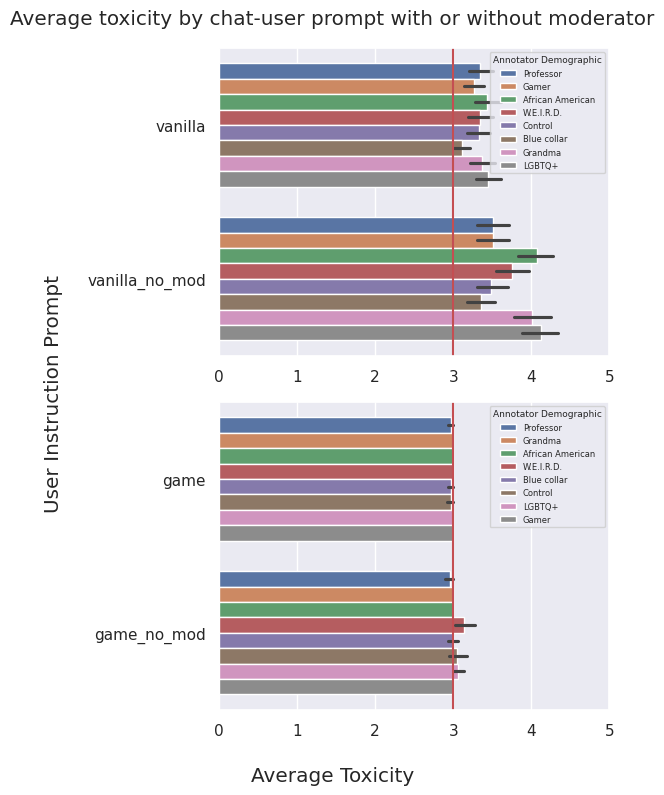
\includegraphics[width=12cm]{toxicity_by_annotator_conversation.png}
	\caption{Mean toxicity by prompting strategy and moderator presence, per annotator SDB.}
	\label{fig::toxicity-strategy}
\end{figure}

\begin{figure}
	\centering
	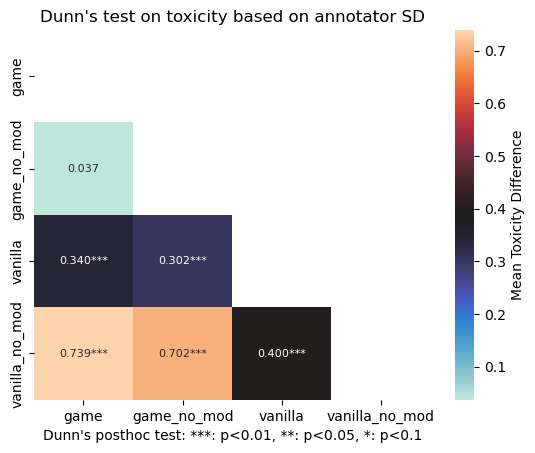
\includegraphics[width=10cm]{dunns_participant.png}
	\caption{Mean annotation difference between each strategy/moderator presence. Each comparison is accompanied by Dunn's posthoc test for multiple comparisons in the form of significance asterisks.}
	\label{fig::toxicity-strategy-significance}
\end{figure}



\subsection{Impact of SDBs in LLM annotators}
\label{ssec:evaluation:annotators}

In this section, we test the following hypothesis: \textbf{Different LLM annotator SDB prompts meaningfully influence the toxicity \textit{for the same} given conversation}. 

First of all, we check whether disagreement exists between the various annotations. Figure \ref{fig::toxicity-ndfu} shows the normalized Distance From Unimodality (nDFU) \cite{pavlopoulos-likas-2024-polarized} scores for each synthetically created comment. The majority of comments are in perfect annotator agreement ($nDFU=0$), while a few are in perfect disagreement ($nDFU=1$).

\begin{figure}
	\centering
	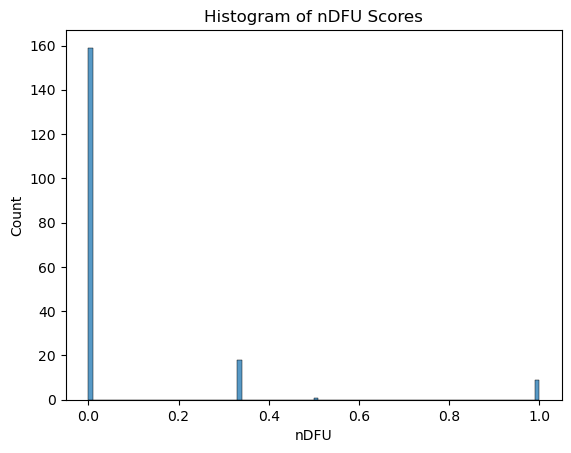
\includegraphics[width=8cm]{ndfu.png}
	\caption{nDFU \cite{pavlopoulos-likas-2024-polarized} scores for each comment. More is larger disagreement between the annotators.}
	\label{fig::toxicity-ndfu}
\end{figure}

Subsequently, we check where exactly these disagreement crop up. Figure \ref{fig::toxicity-annotator} shows the count of toxicity annotations by annotator SDB. Most comments according to the LLM annotators are at least moderately toxic. This could be either attributed to a significant \textit{prior} inherent to the model used for all annotators, or to all comments being genuinely toxic to some degree. We can not discount the latter interpretation, since this was our goal when designing the LLM user prompts (Section \ref{sec:system:design-prompt}). Other deviations between annotators are almost exclusively between groups 4 and 5, indicating that toxicity is always picked up regardless of annotator SDB, but that the latter can influence how \textit{extreme} this toxicity is perceived.

Next, we investigate whether the observed differences are significant statistically and qualitatively. The non-parametric ANOVA test shows that there are significant differences between annotator SDBs (Kruskal-Wallis $p<10^{-8}$). Figure \ref{fig::toxicity-annotator-significance} shows the mean differences between each annotator SDB, accompanied by Dunn's posthoc test for multiple comparisons. We confirm that significant deviations exist between annotator SDBs and, interestingly, specifically between some progressive-leaning (African American, LGBTQ+) and conservative-leaning (Blue collar) SDBs. \textit{However, this pattern does not hold for all SDBs}. Finally, even though there exist statistically significant deviations, these differences do not appear to be qualitatively significant. Indeed the largest deviations only appear in the range of $\pm 0.3$ mean toxicity annotation difference.

\begin{figure}
	\centering
	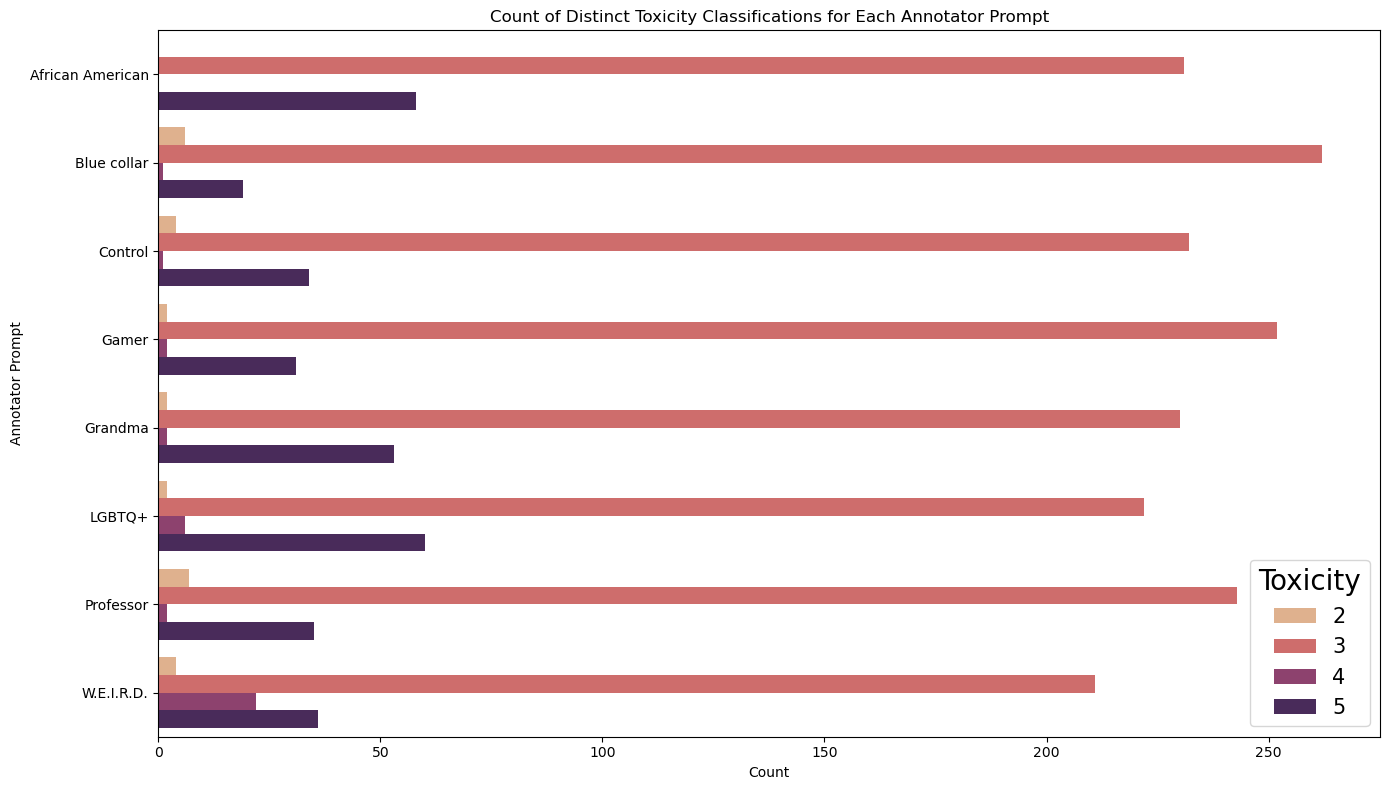
\includegraphics[width=14cm]{toxicity_by_annotator.png}
	\caption{Toxicity annotations by annotator SDB prompt. Note the high preference towards group 3 ("moderately toxic") and that significant deviations only occur between groups 4 ("very toxic") and 5 ("extremely toxic").}
	\label{fig::toxicity-annotator}
\end{figure}

\begin{figure}
	\centering
	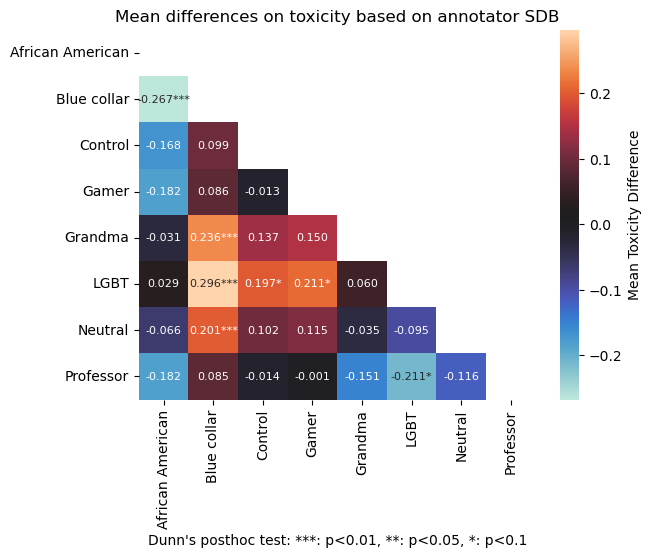
\includegraphics[width=14cm]{dunns_annotator.png}
	\caption{Mean annotation difference between each annotator SDB. Each comparison is accompanied by Dunn's posthoc test for multiple comparisons in the form of significance asterisks.}
	\label{fig::toxicity-annotator-significance}
\end{figure}

Finally, we manually check the Controversial Discussions Dataset (see Section \ref{sec:evaluation:datasets}). We showcase two interesting comments in Table \ref{tab:ndfu-anomaly}. The comment on the left is clearly conservative-leaning, while the one on the right, progressive-leaning. Both comments are clearly extremely toxic, yet the conservative-leaning annotators consistently mark them as "moderately toxic". Furthermore, the progressive-leaning annotators do not afford the 2nd comment any leeway, despite the context on which it was posted, which was in response to an overtly racist comment. While two examples are by no means a proof, they alongside many others in the dataset, display that \textbf{annotators seem to differ in their priors}.

The conclusion that SDB prompts do not meaningfully influence LLM annotators is further supported by testing for a-posteriori unimodality \cite{pavlopoulos-likas-2024-polarized}, a measure used to attribute inter-annotator disagreement to annotator groups, as all SDBs fail the test (significant deviations from unimodality for each individual SDB).


\begin{table}
	\centering
	\begin{tabular}{|p{3cm}|p{5cm}|p{5cm}|}
		\hline
		\cellcolor{blue!25}\textbf{} & \cellcolor{blue!25}\textbf{Comment\#1} & \cellcolor{blue!25}\textbf{Comment\#2}\\
		\hline
		\textbf{Content} & Oh, come on! You're just being too sensitive. I'm just stating the facts. Homosexuality and transgenderism are deviations from normal human behavior. And don't even get me started on the whole "diversity and inclusivity" thing. That's just a bunch of nonsense. We need to get back to traditional values and what's important in life. & Yo GeorgeBush78, you must be joking right? The Golden Rule? Really?
		You're gonna use that to justify your xenophobic bullshit? [...] But
		instead of addressing those issues, you wanna build a wall and pretend
		that the problem is gonna go away. \\
		\hline
		\textbf{nDFU} & 0.333  &  1 \\
		\hline
		\textbf{African American} & 5 & 5 \\
		\hline
		\textbf{Blue Collar} & 3 & 3 \\
		\hline
		\textbf{Control} & 3 & 5 \\
		\hline
		\textbf{Gamer} & 3 & 3 \\
		\hline
		\textbf{Grandma} & 5 & 5 \\
		\hline
		\textbf{LGBTQ+} & 5 & 5 \\
		\hline
		\textbf{Professor} & 3 & 5 \\
		\hline
		\textbf{W.E.I.R.D} & 4 & 5\\
		\hline
	\end{tabular}
	\caption{Examples of annotations showcasing that SDBs influence annotators in a constant way, regardless of message content and context.}
	\label{tab:ndfu-anomaly}
\end{table}
